\documentclass{beamer}
%\usepackage{fancyvrb}
%%%% 和文用 %%%%%
%\usepackage{bxdpx-beamer} % dvipdfmxで下のボタンを機能させる
%\usepackage{pxjahyper} % 日本語でしおり機能を使う
%\usepackage{minijs} % フォントメトリックをmin10 -> minijs
\usepackage{hyperref} % リンクを機能させる
%\renewcommand{\kanjifamilydefault}{\gtdefault} % 既定和文フォントをゴシック体にする
\usepackage{xltxtra}


%%%% スライドの見た目 %%%%%
\usetheme{Berlin}
\usefonttheme{professionalfonts}
\setbeamertemplate{navigation symbols}{}
\setbeamertemplate{frametitle}[default][center]
% \setbeamercovered{transparent}%好みに応じてどうぞ)
\setbeamertemplate{footline}[frame number] % ページ番号表示
\setbeamercolor{page number in head/foot}{fg=gray} % ページ番号の色

% \setbeamerfont{footline}{size=\normalsize,series=\bfseries}
%\setbeamercolor{footline}{fg=black,bg=black}
% \pagestyle{empty}
%%%%

	
	\usepackage{tipa} 									% phonetic signs
	\usepackage{fontspec}      							% Apparently defines most aliases from TIPA.
	\usepackage{xunicode}								% to use Unicode codes	
		\usepackage{xltxtra}
	\usepackage{gb4e}									% for glossed examples
    
%%%% 定義環境 %%%%%


	\usepackage{tipa} 									% phonetic signs
	\usepackage{fontspec}      							% Apparently defines most aliases from TIPA.
	\usepackage{xunicode}								% to use Unicode codes	

	\usepackage{xltxtra}
	\usepackage{gb4e}									% for glossed examples


	

% Custom font for a frame.
%\newcommand{\customframefont}[1]{
%\setbeamertemplate{itemize/enumerate body begin}{#1}
%\setbeamertemplate{itemize/enumerate subbody begin}{#1}
%}

%\NewEnviron{framefont}[1]{
%\customframefont{#1} % for itemize/enumerate
%{#1 % For the text outside itemize/enumerate
%\BODY
%}
%\customframefont{\normalsize}
%}
%%%%%%%%%


 
\title[Building Web Corpus of Old Nubian with Interlinear Glossing by Miyagaw and van Gerven Oei, JADH2021]{Building Web Corpus of Old Nubian with Interlinear Glossing as Digital Cultural Heritage for Modern-Day Nubians}
\author[]{So Miyagawa and Vincent W.J. van Gerven Oei}
\institute[]{Kyoto University, Punctum Books \& Coventry University}
\date{\today}

\begin{document}

\begin{frame}
\titlepage %表紙
\end{frame}

\begin{frame}\frametitle{Contents}
	\tableofcontents %目次
\end{frame}

\section{Old Nubian}

\begin{frame}{The Old Nubian language}
  \begin{itemize}
    \item A Nubian language
    \item Recorded in the kingdoms of Nobadia and Makuria in the Middle Nile Valley 
    \begin{itemize}
      \item Modern-day southern Egypt and northern Sudan
      \item Between the 8th and 15th centuries CE 
    \end{itemize}
  \end{itemize}
 \begin{center}
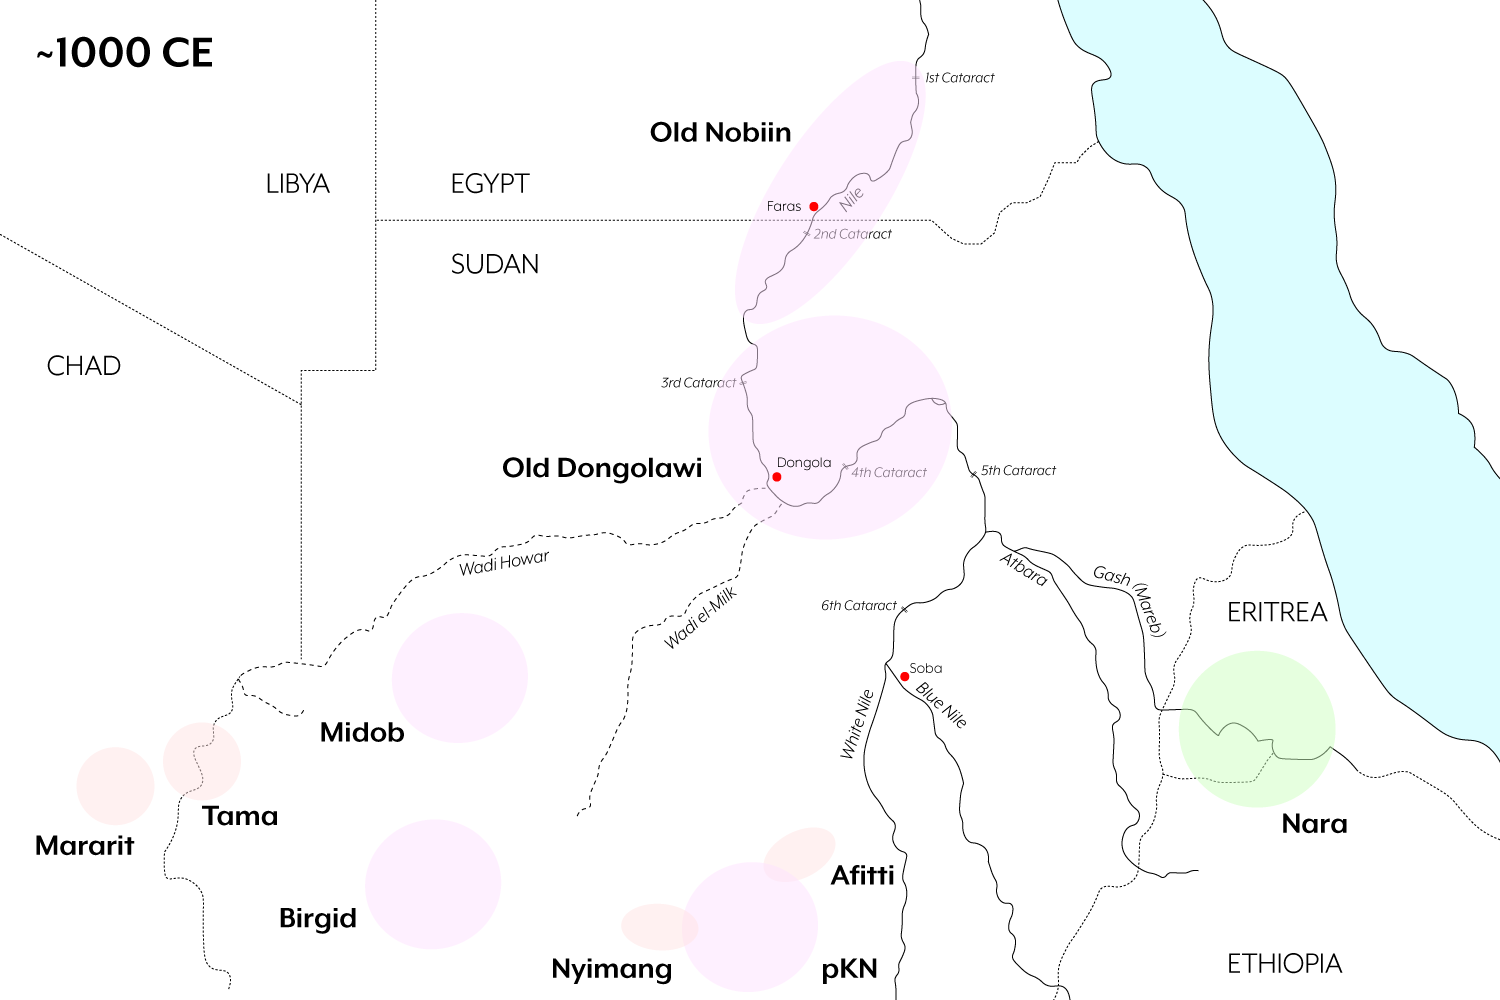
\includegraphics[width=0.8\textwidth]{1000CE.png}
\end{center}
\end{frame}

\begin{frame}{The Nubian alphabet}
  \begin{block}{Second oldest in Nilo-Saharan}
    Besides Meroitic, Old Nubian is the oldest written language from the Nilo-Saharan language 
    phylum.
  \end{block}
  \begin{itemize}
    \item Written using the Coptic-derived Nubian alphabet
    \item Coptic alphabet: Greek alphabet + 6-7 Demotic-derived letters
    \item Includes three characters from the Meroitic alphasyllabary
  \end{itemize}
\begin{center}
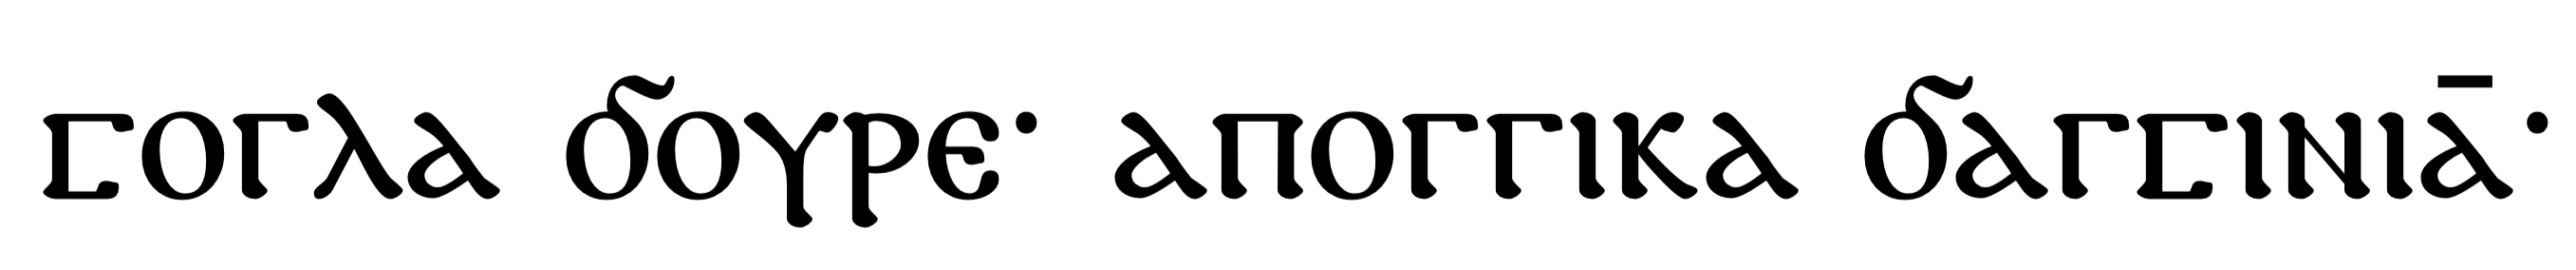
\includegraphics[width=1.0\textwidth]{ontext.png}
\end{center}
\end{frame}

\begin{frame}{Old Nubian texts}
  \begin{itemize}
    \item Old Nubian corpus consists of both 1. literary material and 2. documentary materials
    \begin{enumerate}
      \item Such as Bible translations and sermons, and burial texts
      \item Such as contracts, land sales, wall inscriptions
    \end{enumerate}
  \end{itemize}
  \begin{center}
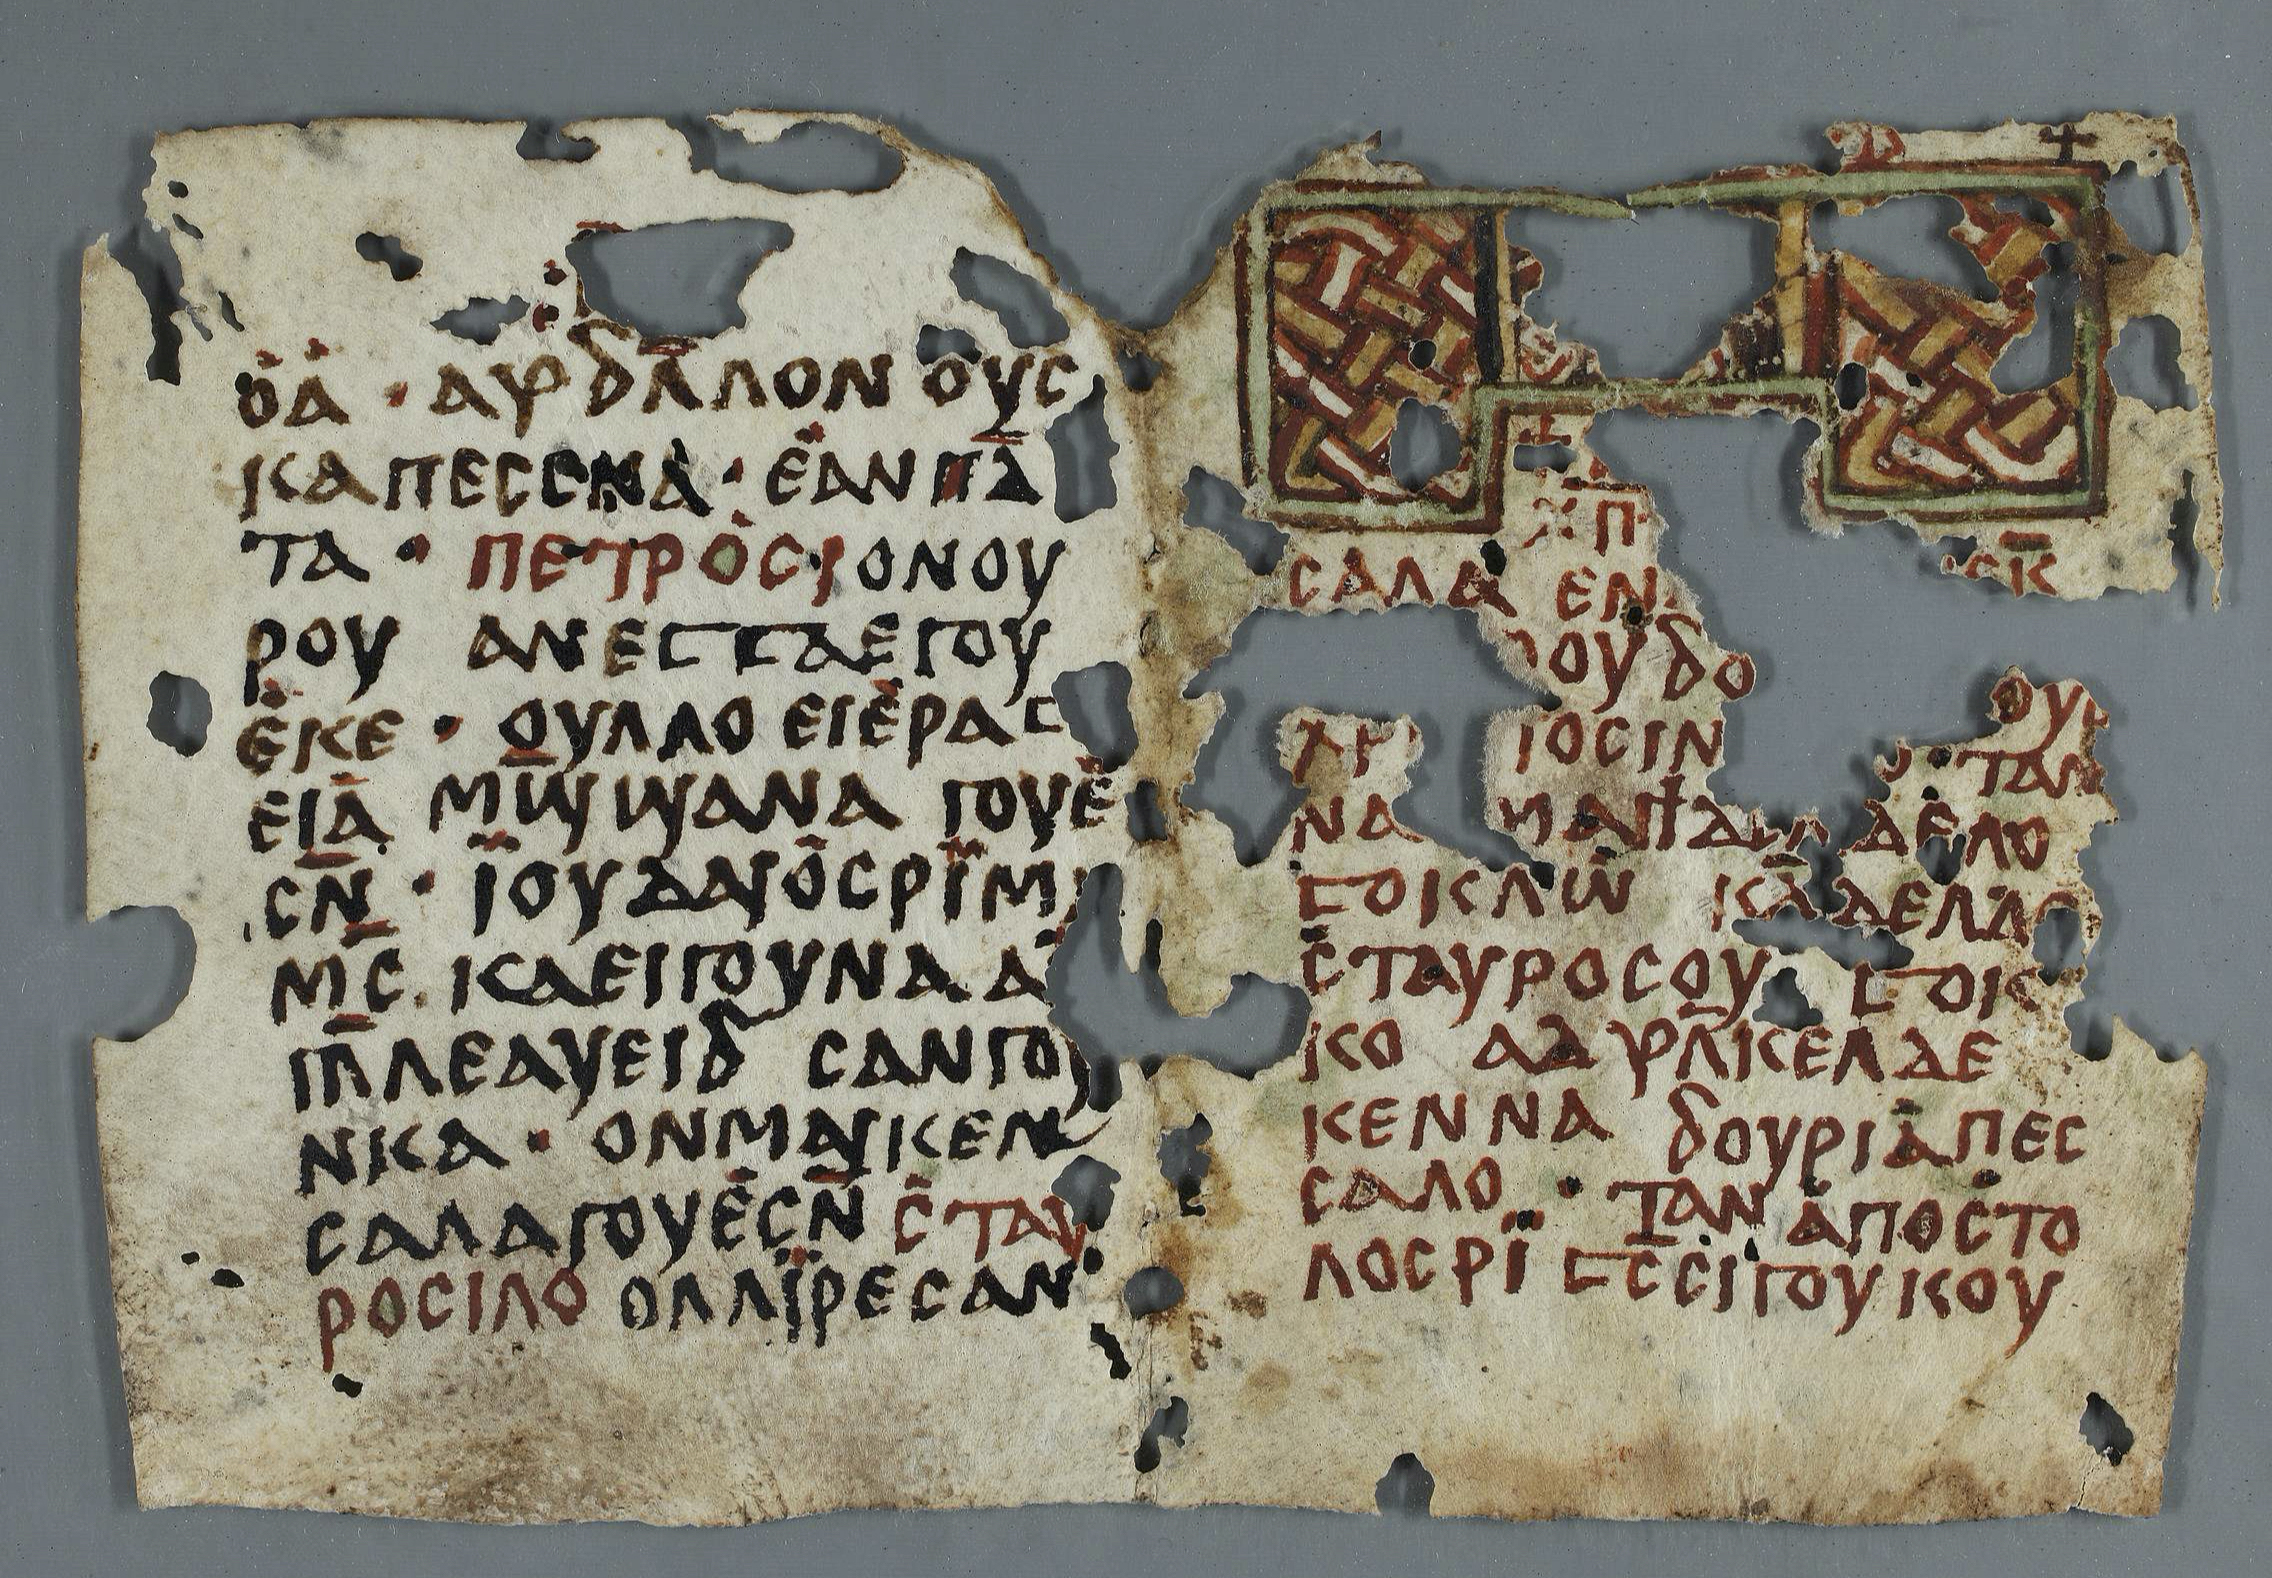
\includegraphics[width=0.7\textwidth]{St-f2r.jpg}
\end{center}
\end{frame}

\section{Goal of the project}

\begin{frame}{Project goal}
  \begin{alertblock}{Problem so far...}
    There is no digital text corpus of Old Nubian.
   \end{alertblock}
   \begin{exampleblock}{Team for the Digital Old Nubian Corpus project}
      \begin{description}
          \item[So Miyagawa] digital humanist and Coptologist 
          \item[Vincent van Gerven Oei] Old Nubian language expert
      \end{description}
  \end{exampleblock}
  \begin{block}{Our goal: linguistically and philologically tagged corpus}
    \begin{itemize}
      \item User-friendly, highly visual online digital platform
      \item Data sustainability and interoperability through TEI XML
    \end{itemize}
  \end{block}
\end{frame}

\begin{frame}{Linguistic tagging for Old Nubian texts}
  \begin{itemize}
    \item Visualization for both linguistic experts and Nubian heritage holders
    \begin{enumerate}
      \item For linguists, interlinear glosses following Leipzig Glossing Rules (LGR)
       \begin{itemize}
          \item Glosses under each word and morpheme
        \end{itemize}
        \item For Modern-Day Nubians, Arabic and plain English grammatical annotations 
        \begin{itemize}
          \item Nubians: heritage holders of Old Nubian
        \end{itemize}
     \end{enumerate}
  \end{itemize}
  \begin{center}
  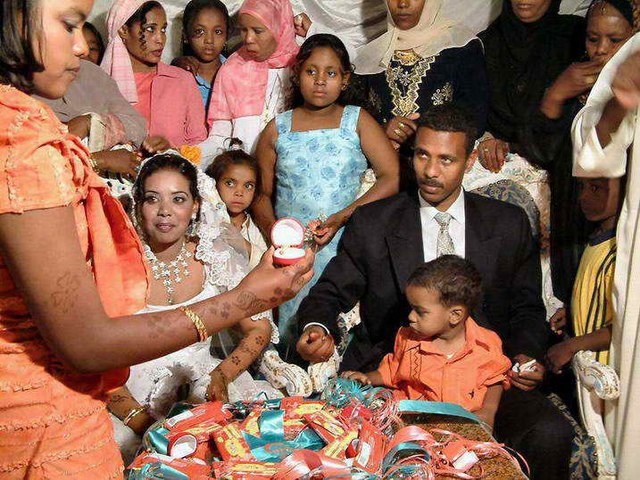
\includegraphics[width=0.4\textwidth]{nubian.jpg} 
\\ {\tiny Sms, CC BY-SA 3.0}
\end{center}
\end{frame}

\section{Corpus-building methodology}

\begin{frame}{Corpus-building methodology}
  \begin{block}{Corpus data originally composed in \XeLaTeX}
    Interlinear glossing realized in four lines by gb4e.sty 
    \begin{enumerate}
      \item Old Nubian text in the Old Nubian alphabet 
      \item Romanized version of the same Old Nubian text 
      \begin{itemize}\item Morphemes parsed by hyphens \end{itemize}
      \item Interlinear glossing
      \item  English translation
    \end{enumerate} 
  \end{block}
\begin{center}
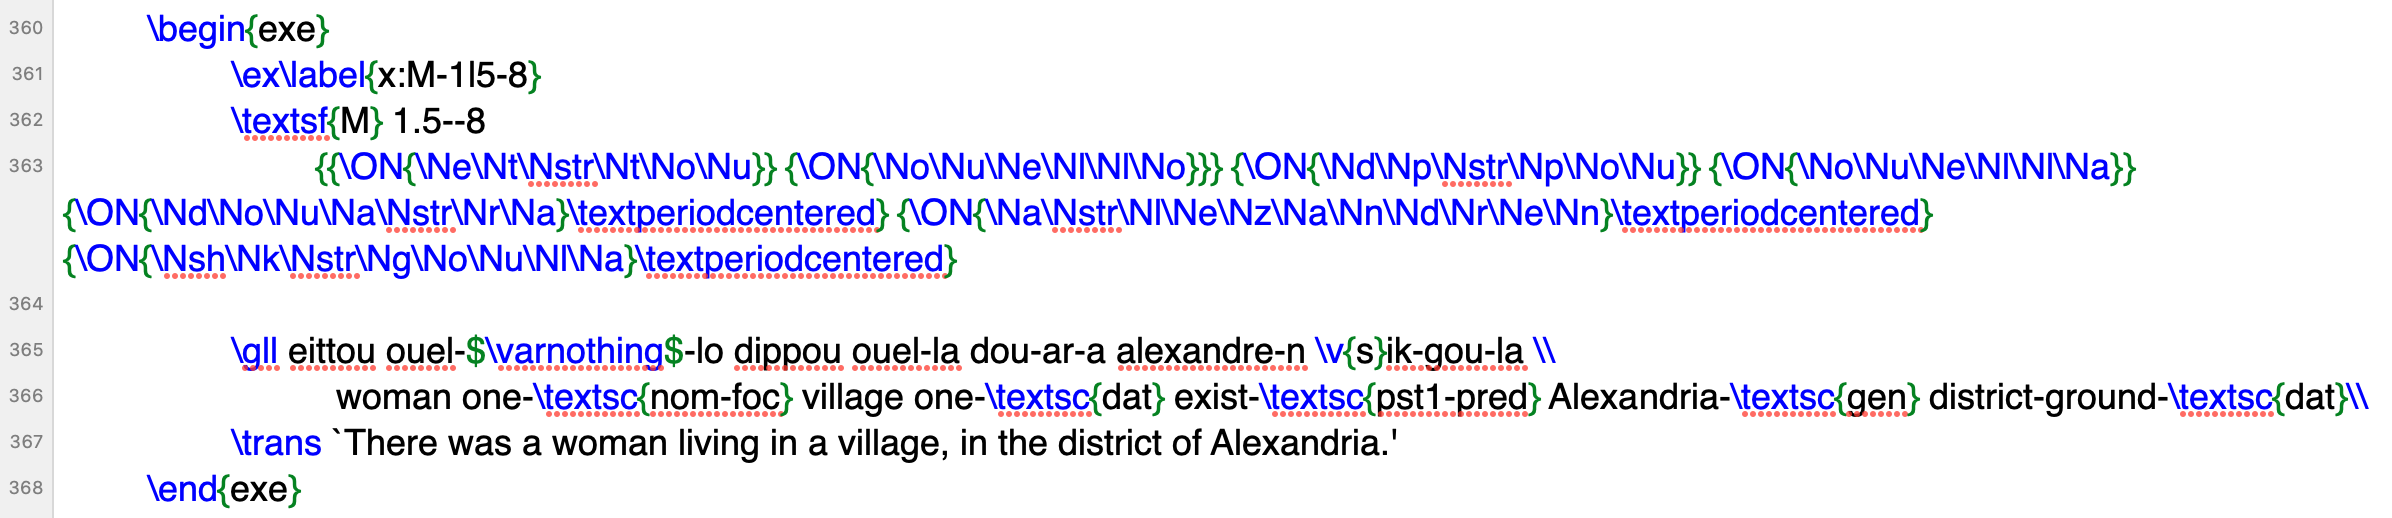
\includegraphics[width=1.0\textwidth]{xelatex.png}
\end{center}
\end{frame}

\begin{frame}{The entire Old Nubian corpus}
\begin{itemize}
\item The entire Old Nubian corpus is not as big as that of Coptic and far smaller than that of Ancient Greek 
\item Large amounts of epigraphic materials 
\item The most sizable is Pseudo-Chrysostomus’s {\it In venerabilem crucem sermo}: ~3,200-word 
\item The second most sizable text is {\it the Miracle of Saint Mina}: ~950 words. 
\end{itemize}
\end{frame}

\section{Pilot project}

\begin{frame}{Starting point}
  \begin{block}{Pilot project of digital Old Nubian corpus}
    \begin{itemize}
      \item Stauros Text:  ~800 words, relatively long
      \item Vincent van Gerven Oei developed the interlinear glossed text file in XeLaTeX
      \item So Miyagawa created XSLT to convert this XeLaTeX file into TEI XML format
   \end{itemize}
  \end{block}
  \begin{center}

\end{center}
  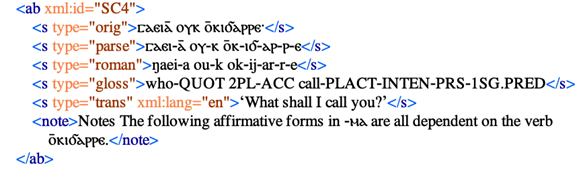
\includegraphics[width=0.9\textwidth]{tei.png}
\end{frame}

\begin{frame}{Making it into a webpage}
  \begin{columns}
    \begin{column}{0.6\textwidth}
  \begin{itemize}
    \item XSLT program to transform the TEI XML into an HTML file 
    \item Combined with a JavaScript file (leipzig.js by Benjamin Chauvett) 
    \item to enable visualization of our interlinear glosses in the form of LGR 
    \item This pipeline produced the first online Old Nubian corpus
  \end{itemize}

    \end{column}
    \begin{column}{0.4\textwidth}
    \begin{center}
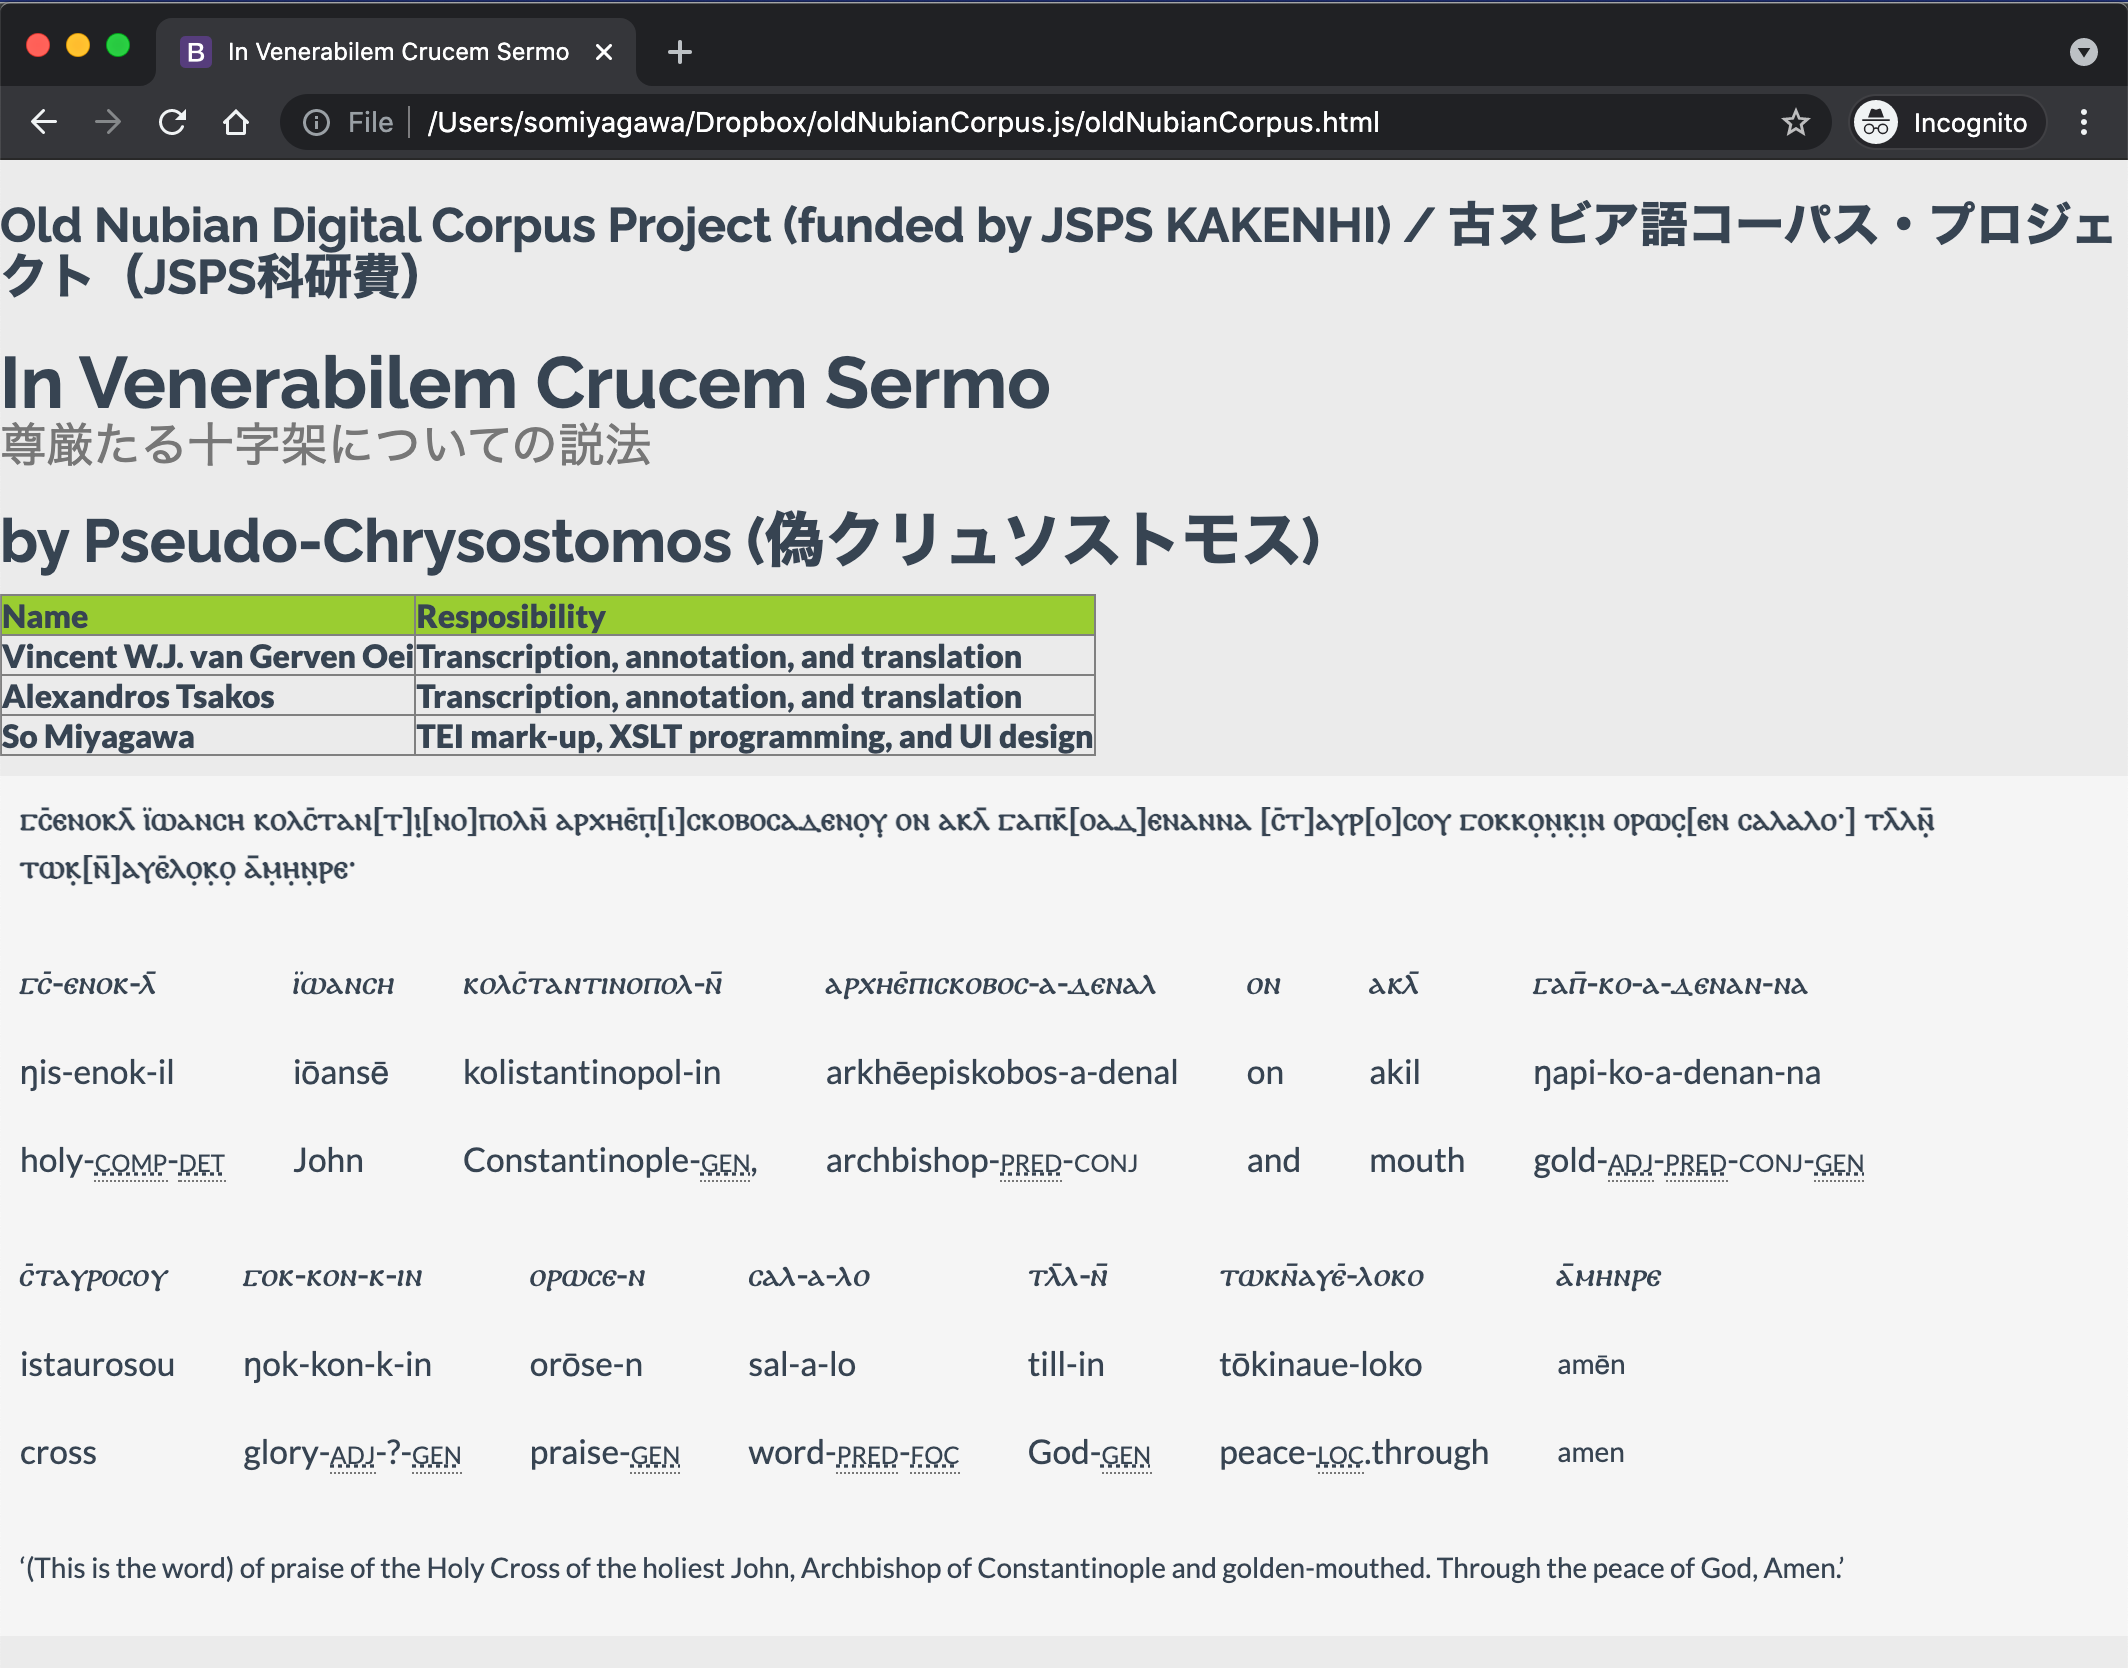
\includegraphics[width=1.0\textwidth]{webcorpus.png} 
\\
       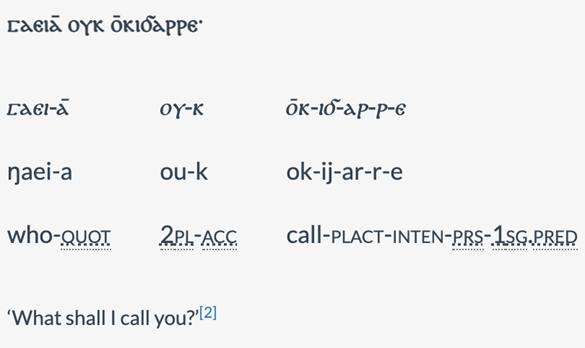
\includegraphics[width=1.0\textwidth]{webpage.png}
\end{center}

    \end{column}
\end{columns}



\end{frame}
 

\section{Future perspectives for digital cultural heritage}

\begin{frame}{Future perspectives for digital cultural heritage 1}
   \begin{itemize}
      \item More Old Nubian literary texts with LGR-styled interlinear glossing via TEI 
      \item To facilitate an online search, we will create a search function of each lemmata and 
      glosses on the homepage using XQuery
      \item Providing photos of Old Nubian manuscripts in IIIF
      \item First digitized lexicon data of Old Nubian for further NLP development for Old Nubian
   \end{itemize}
\begin{center}
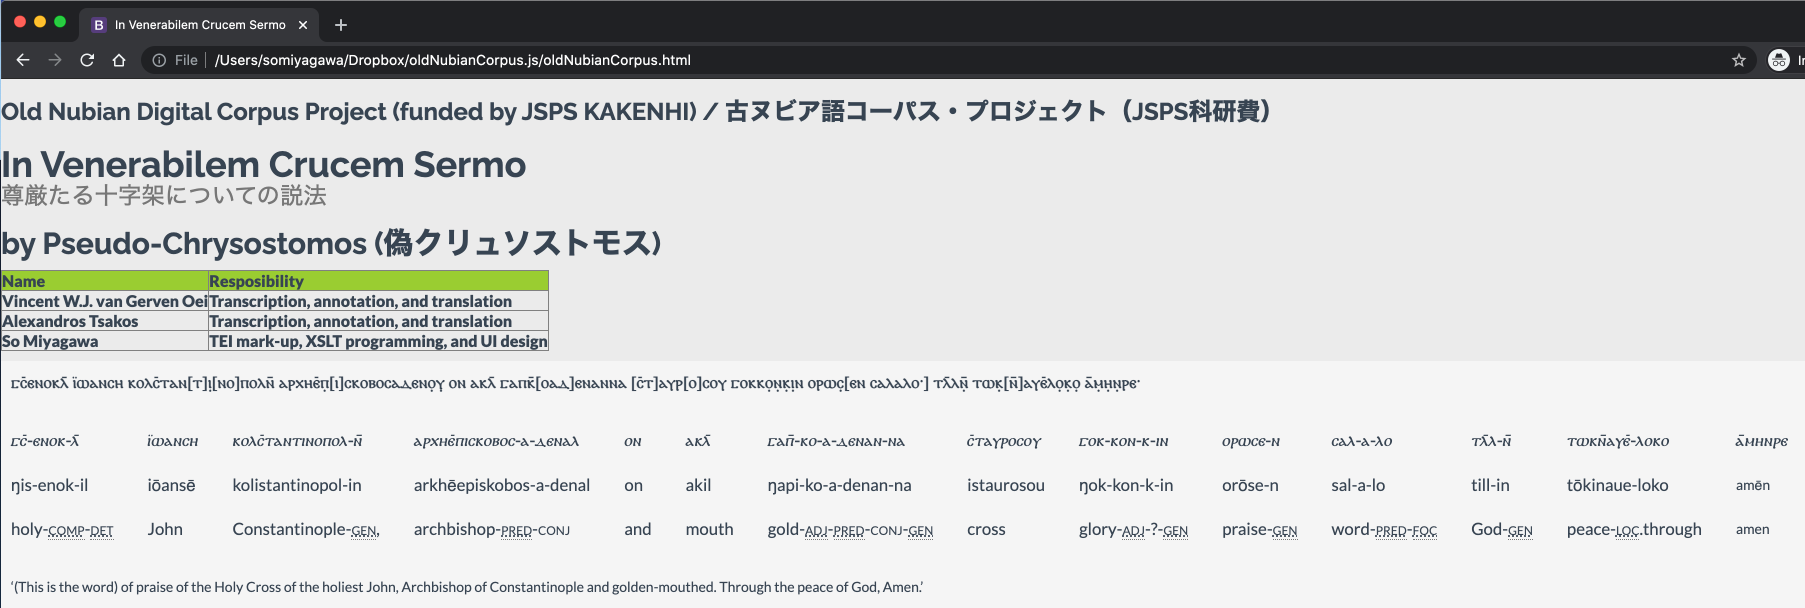
\includegraphics[width=1.0\textwidth]{webcorpus2.png}
\end{center}

\end{frame}

\begin{frame}{Future perspectives for digital cultural heritage 2}
    \begin{itemize}
      \item Primarily aimed at Old Nubian philology experts or linguistics, or historians in 
      Medieval Nubia 
      \item But planning to embed 
      \begin{itemize}
        \item plain English and Arabic translations
        \item easy-to-read explanations for each gloss
        \item a basic grammar of Old Nubian
        \item lecture videos
      \end{itemize}
      \item To contribute to Nubian cultural preservation and heritage education 
      \item To spread knowledge of the Nubian culture to a wider global audience.
   \end{itemize}
\end{frame}


%\section{楕円曲線暗号とは}


%\begin{frame}\frametitle{Old Nubian (古ヌビア語)}
%\begin{block}{A Nilo-Saharan language}
%\begin{itemize}
 %\item Nilo-Saharan(?) $>$ East Sudanic $>$ North East $>$ Nubian $>$ Nile Nubian $>$ Old Nubian
 %\item 8 -- 15 AD
 %\item SOV, suffixal, noun -- adjective, agglutinative language

 
%\end{itemize}
%\end{block}
% picture of glosses of V
%\end{frame}

% Christian culture in Three Medieval Nubian Kingdoms
%\begin{frame}\frametitle{Written in Coptic alphabet with three Meroitic Demotic}
%\centering
%\begin{eqnarray}
%i\rho^{\prime}=U\left(  i\rho\right)  U^{\dagger}=Ad_{U}\left(  i\rho\right)\\
%i\rho^{\prime}=Ad_{U}\left(  i\rho\right)  =U\left(  i\rho\right)  U^{-1}%
%\end{eqnarray}
%\vspace{16pt}
%\href{http://www.csee.umbc.edu/~lomonaco/ams/lecturenotes/figssamtangle/unusedfigs/samtangle.tex}{ref: An Entangled Tale of Quantum Entanglement}%\end{frame}

\end{document}
